\documentclass[11pt,a4paper]{report}
\usepackage[utf8]{inputenc}
\usepackage{amsmath}
\usepackage{amsfonts}
\usepackage{amssymb}
\usepackage{makeidx}
\usepackage{graphicx}
\usepackage[left=4.00cm, right=3.00cm, top=3.00cm, bottom=3.00cm]{geometry}
\usepackage[bahasa]{babel}

\begin{document}
	\begingroup
	\thispagestyle{empty}  
	\begin{center}
		%TITLE
		\textbf{
			\Large
			Na\"{i}ve Bayes untuk Klasifikasi Data : Studi Kasus Car Dataset\\[1cm]
			\normalsize
			Laporan Tugas Besar	
			\\[1cm]
			%AUTHOR
			Rizki\\
			Mirza Dita A\\
			Ali Ridho F\\
			Luthfi Rendragiri
			\\[2cm]
			%LOGO
			
\includegraphics[width=0.35\linewidth]{logo}\\[2cm]
			%UNIVERSITY
			\Large
			Program Studi Sarjana Teknik Informatika\\
			Fakultas Informatika\\
			Universitas Telkom\\
			Bandung\\[0.2cm]
			2015}
	\end{center}
	\endgroup
	\newpage
	\chapter{Dasar Teori}
	\section{Teorema Bayes}
	Teorema bayes, Hukum Bayes, atau Aturan Bayes merupakan teorema yang ditemukan oleh Thomas Bayes, ahli statistika dan filosofis Inggris.Teorema Bayes berkaitan tentang probabilitas kondisional. Secara umum, teorema Bayes dapat dinyatakan dengan persamaan matematis sebagai berikut :
	\[ P(A|B)=\frac{P(B|A)P(A)}{P(B)} \]
	Dimana A dan B merupakan \emph{event}.
	\begin{itemize}
		\item $P(A)$ dan $P(B)$ merupakan peluang tiap masing-masing \emph{event}.
		\item $P(A|B)$ merupakan probabilitas kondisional untuk $A$ jika $B$ terjadi.
	\end{itemize} 
	
	Pada kecerdasan artifisial dan \emph{Data Mining}, teorema Bayes digunakan dalam metode \emph{learning} yang sering disebut dengan nama \emph{Na\"{i}ve Bayes Classifier}. Pada beberapa referensi, algoritma ini memiliki penamaan yang beragam.
	
	Implementasi didunia nyata cukup beragam, misal untuk \emph{text classification}, \emph{spam filtering}, \emph{document classification}, dan lain-lain. Berikut contoh sederhana untuk \emph{Na\"{i}ve Bayes Classifier} : 
	\subsection{Contoh}
	Misal, terdapat dua kelas yaitu,
	\[ c1=pria, c2=wanita \]
	diketahui, ada orang bernama "Drew" yang jenis kelaminnya diasumsikan kita tidak tahu. Berdasarkan kelas yang ada, probabilitas yang mungkin adalah, $P(pria|drew)$ atau $P(wanita|drew)$.
	Misal kita memiliki data sebagai berikut:
	
	\begin{table}[h]
		\centering
		\begin{tabular}{|c|c|}
			\hline Nama & Jenis Kelamn \\ 
			\hline Drew & Pria \\ 
			\hline Claudia & Wanita \\ 
			\hline Drew & Wanita \\ 
			\hline Drew & Wanita \\ 
			\hline Alberto & Pria \\ 
			\hline Karin & Wanita \\ 
			\hline Sergio & Pria \\ 
			\hline 
		\end{tabular}
		\caption{Data sampel acak}
	\end{table} 
	
	Diketahui berdasarkan Teorema Bayes,
	\[ P(A|B) = \frac{P(B|A)(P(A)}{P(B)}\]
	sehingga, dengan data yang kita miliki,
	\[ P(pria|drew) = \frac{1/3*3/8}{5/8}=\frac{0.125}{0.625}=0.2\]
	\[ P(wanita|drew) = \frac{2/5*5/8}{3/8}=\frac{0.250}{0.667}=0.374\]
	Maka, berdasarkan sampel acak dari tabel diatas, orang yang bernama Drew besar kemungkinan berjenis kelamin wanita.
	\newpage
	\chapter{Program dan Algoritma}
	\section{Algoritma}
	Pada kasus tugas besar ini, digunakan dataset yang telah diberikan (\emph{car.dat}) yang kemudian akan dibagi menjadi dua bagian yaitu data training dan data testing. Misal, 20\% data testing 80\% data training, atau kombinasi lain.
	
	Algoritma komputasi pada program yang telah dibuat dapat dilihat pada method berikut:
	\begin{description}
		\item[calcProbIndependent] menghitung \emph{independent probability} pada kelas tertentu terhadap data training.
		\item[CalcDependentProb] menghitung \emph{dependent probability} atribut tertentu terhadap kelas tertentu. Dipanggil pada method \emph{calcDependentOne}
		\item[CalcDependentOne] menghitung \emph{dependent probability} untuk satu \emph{record} (seluruh atribut) terhadap seluruh kelas.
		\item[calcTotalDependent] menghitung jumlah \emph{dependent} suatu atribut terhadap kelas tertentu di data training. Dipanggil pada method \emph{calcDependentProb}
		\item[calcRecordTotal] menghitung jumlah \emph{record} yang ada pada data training. Dipanggil pada method \emph{calcDependentProb}
		\item[classification] mengklasifikasikan suatu \emph{record} pada kelas tertentu.
		\item[calcAccuracy] menghitung akurasi hasil klasifikasi. 
	\end{description}
	\subsection{Algoritma Independent Probability}
	Berdasarkan pada method \emph{calcProbIndependent}, algoritma untuk menghitung probabilitas independen adalah sebagai berikut:
	\[ P(kelas) = \frac{nKelas}{nData}\]
	\begin{itemize}
		\item nData adalah banyaknya datatraining.
	\end{itemize}
	Contoh : 50\% data training, sehingga \emph{independent probability} yang didapat adalah sebagai berikut:
	\[ P(unacc) = \frac{180}{864}=0.2083\]
	\[ P(acc) = \frac{684}{864}=0.7916\]
	\[ P(vgood) = \frac{0}{864}=0\]
	\[ P(good) = \frac{0}{864}=0\]
	
	\subsection{Algoritma Dependent Probability}
	Berdasaran pada method \emph{calcDependenProb}, algoritma untuk menghitung probabilitas dependen adalah sebagai berikut:
	\[ P(acc|x)=\frac{P(x_{1}|acc)P(x_{2}|acc)P(x_{3}|acc)P(x_{4}|acc)P(x_{5}|acc)P(x_{6}|acc)P(acc)}{P(x)} \]
	dengan $x$ adalah satu \emph{record} data, dalam kasus ini memiliki enam header / atribut. 
	\newpage
	
	\section{\textit{Class Diagram}}
	\begin{figure}[h]
	\centering
	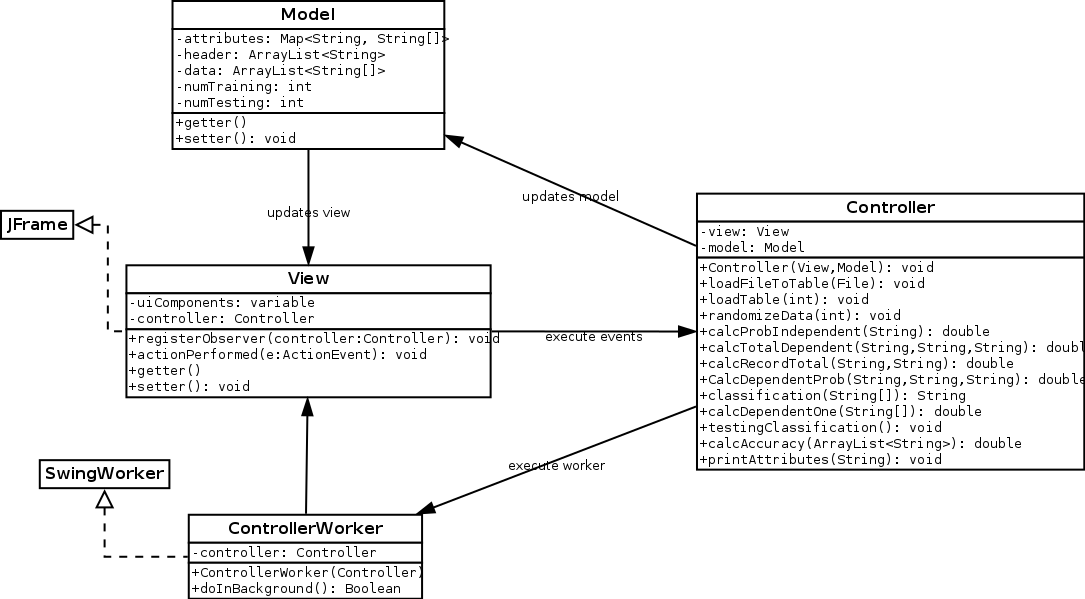
\includegraphics[width=13cm, height=7cm]{class}
	\caption{Class Diagram}
	\label{fig:class}
	\end{figure}
	
	\begin{figure}[h]
	\centering
	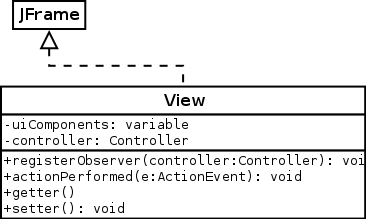
\includegraphics[width=0.5\linewidth]{view}
	\caption{View}
	\label{fig:view}
	\end{figure}
	\newpage
	\begin{figure}[h]
	\centering
	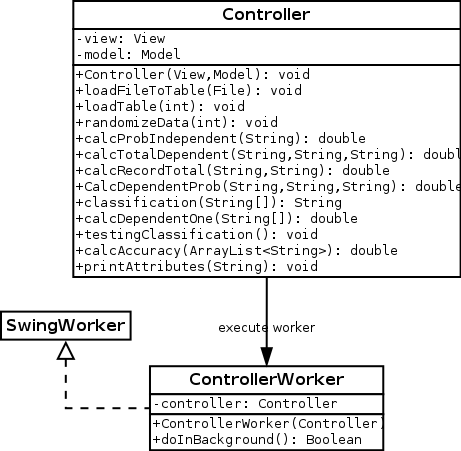
\includegraphics[width=0.7\linewidth]{controller}
	\caption{Controller}
	\label{fig:controller}
	\end{figure}
	
	\begin{figure}[h]
	\centering
	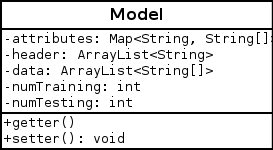
\includegraphics[width=0.5\linewidth]{model}
	\caption{Model}
	\label{fig:model}
	\end{figure}
	\newpage
	\section{Fungsionalitas Program}
	Selain fungsionalitas utama, terdapat fitur tambahan pada program meliputi:
	\begin{itemize}
		\item Tatap muka pengguna dengan \emph{swing}
		\item \emph{Randomize} atau acak data
		\item \emph{Multi-threading} untuk komputasi berat (klasifikasi testing).
		\item \emph{Console verbose} untuk melihat log jalannya program.
		\item \emph{splitting} data training dan data testing dengan \emph{slider}  
		\item \emph{load} dan \emph{save} data dari \emph{dataset} ke basis data dengan MySQL.
	\end{itemize}
	\chapter{Analisis}
	\section{Test Case}
	\begin{figure}[h]
	\centering
	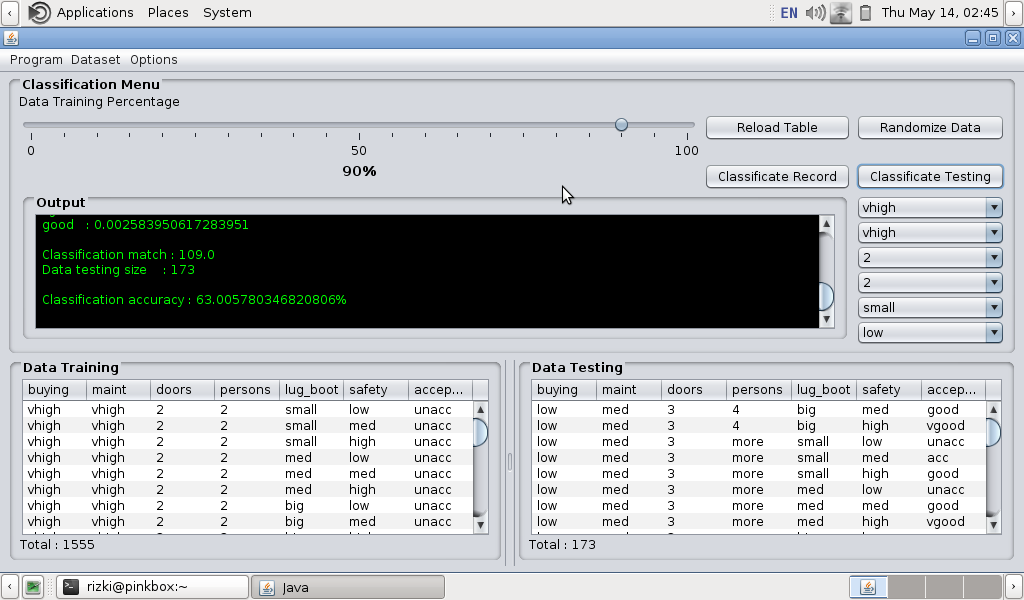
\includegraphics[width=0.7\linewidth]{../results/9010-nonrandom}
	\caption{Testcase 90:10 tanpa acak data}
	\label{fig:9010-nonrandom}
	\end{figure}
	\begin{figure}[h]
		\centering
		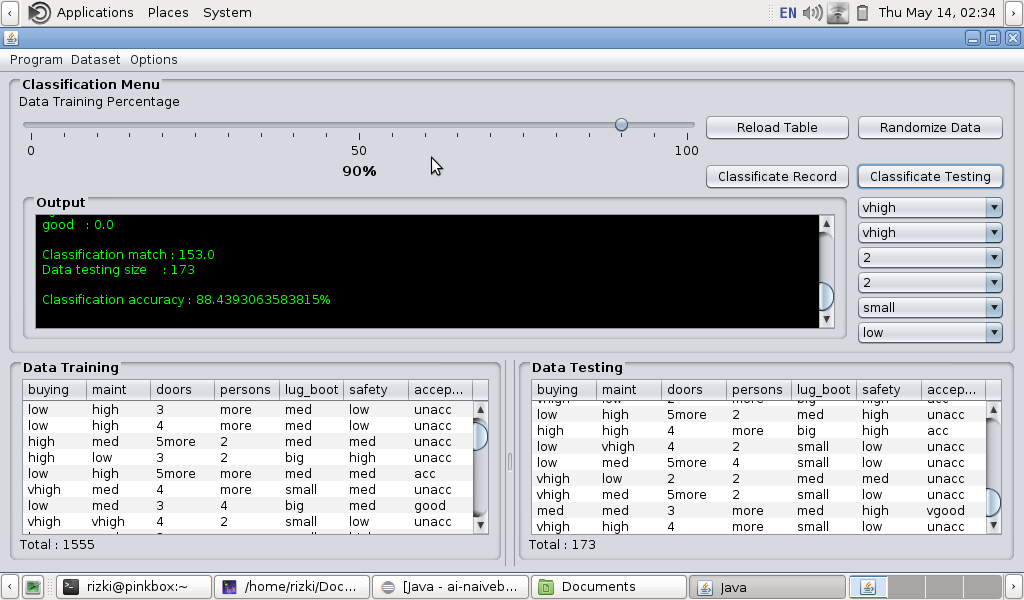
\includegraphics[width=0.7\linewidth]{../results/9010-5}
		\caption{Testcase 90:10 dengan data acak}
		\label{fig:9010-5}
	\end{figure}
	
	Dengan program yang telah dibuat, dilakukan testcase dengan dataset \emph{car.dat} yang telah disediakan. Adapun testcase akan diujikan pada perbandingan datat raining dan data testing sebesar 75:25, 50:50, 25:75, 10:90, dan 90:10. Kemudian akan dilakukan analisis terhadap hasil testcase dan ditentukan saran terhadap permasalahan ini.
	
	Setelah dilakukan testcase sebanyak lima kali untuk masing-masing perbandingan data training dan data testing yang telah diacak, dihasilkan nilai keakuratan yang fluktuatif dengan kisaran rata-rata terletak diantara 80\%-90\%. Namun, akurasi akan sangat buruk jika data tidak diacak. Hal ini normal, karena dataset yang disediakan adalah terurut. Selain itu \emph{splitting} data dilakukan dengan cara membagi data dengan perbandingan yang telah ditentukan. Oleh karena itu, perlu dibuatkan method untuk mengacak data sebelum dilakukannya klasifikasi data testing.
	\section{Kesimpulan dan Saran}
	Berdasarkan hasil pengujian, kesimpulan yang didapatkan yaitu :
	\begin{itemize}
		\item Algoritma \emph{Na\"{i}ve Bayes Classifier} memiliki keakuratan yang cukup baik dengan implementasi yang tidak terlalu sulit.
		\item Urutan data berpengaruh terhadap nilai akurasi.
		\item Nilai akurasi bersifat fluktuatif dengan kisaran rata-rata yaitu antara 80\% hingga 90\%.
		\item Perbandingan ukuran data training dan data testing mempengaruhi nilai akurasi.
	\end{itemize}
	Adapun saran dari hasil pengujian ini antara lain :
	\begin{itemize}
		\item Diperlukan kajian untuk mencari fungsi acak yang menghasilkan nilai akurasi optimal.
		\item Dilakukan klasifikasi dengan metode lain (optimasi algoritma \emph{Na\"{i}ve Bayes Classifier}).
		\item Dilakukan testcase yang lebih banyak agar hasil kajian akurat.
	\end{itemize}
	\newpage
	\chapter*{Lampiran}
	\section*{Catatan}
	\begin{itemize}
		\item kode sumber dapat diunduh di https://github.com/rizkidoank/tugasbesar.
		\item \emph{screenshot} hasil testcase lengkap dapat diunduh di alamat github diatas.
	\end{itemize}
	\section*{Tangkapan Layar}
	\begin{figure}[h]
	\centering
	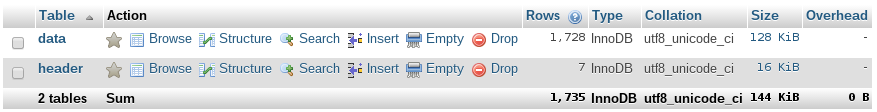
\includegraphics[width=0.7\linewidth]{database}
	\label{fig:database}
	\end{figure}
	\begin{figure}[h]
		\centering
		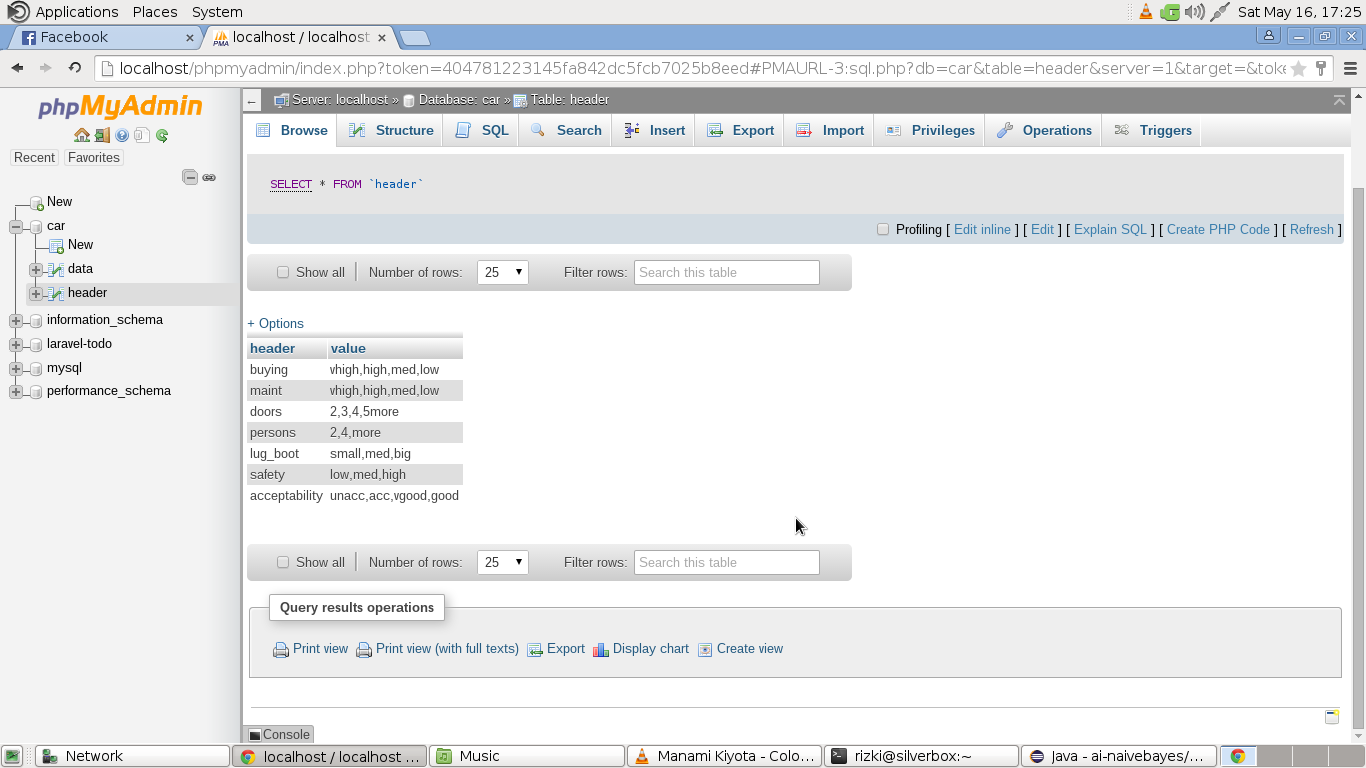
\includegraphics[width=0.7\linewidth]{header}
		\label{fig:header}
	\end{figure}
	\begin{figure}[h]
		\centering
		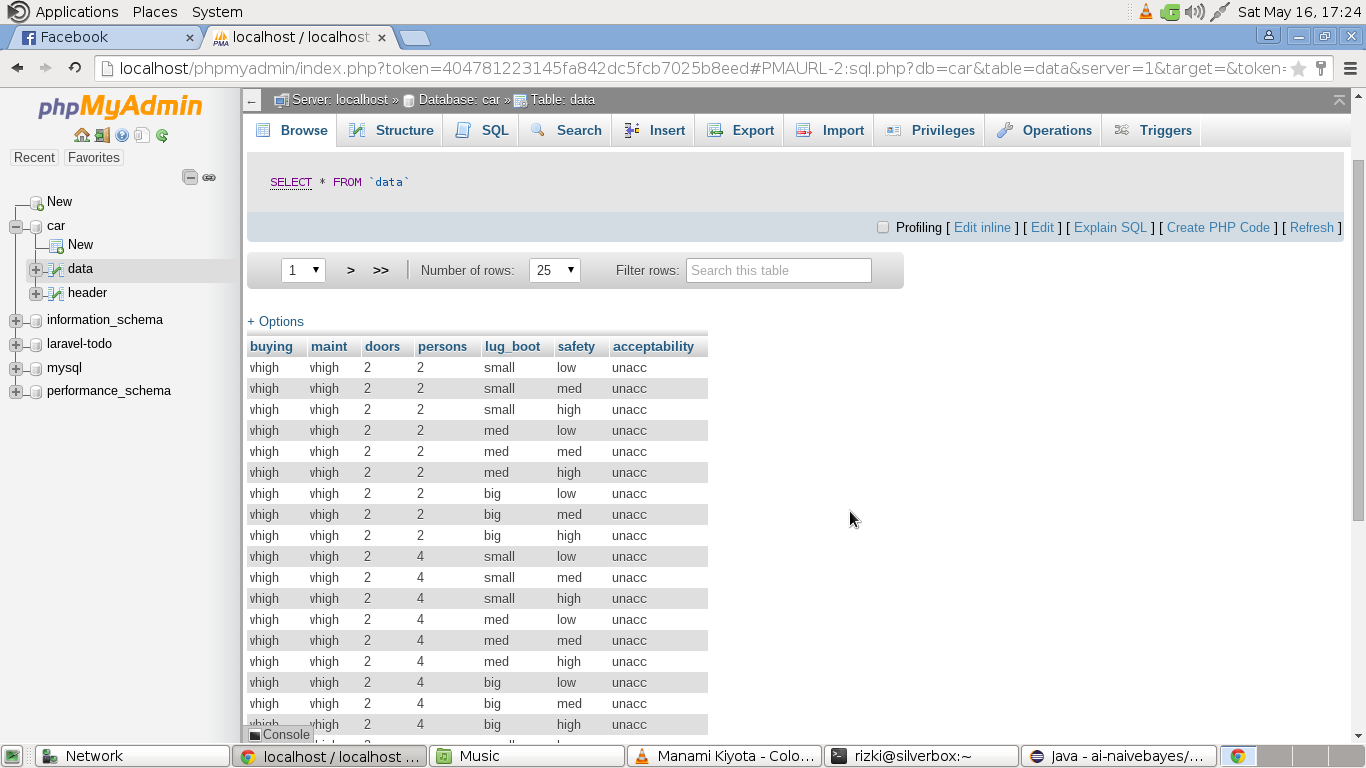
\includegraphics[width=0.7\linewidth]{data}
		\label{fig:data}
	\end{figure}
	\nocite{*}
	\bibliographystyle{IEEEtran}
	\bibliography{referensi}
\end{document}